\section{Non-pipelined Implementation}

For non-pipelined implementation, the arithmetic logic block functions with a clock
and an active low signal LOAD to load the operands A and B into the operand registers.
After finishing the arithmetic operations, the result will be stored in the output register with a high EN\_FLAG signal.
The END\_FLAG signal is used to denote whether the output is valid, it is asserted when the calculation has finished.
The CLEAR signal will clear all the operand and output registers to ‘0’ when it is active high.

\subsection{Operating Circuit}

Once the operands A and B are loaded into the operand registers.
The output of these registers is then fed into the designed multiplier to perform the multiplication calculation required by the arithmetic unit.
The output of the multiplication unit is then fed into the shifter unit.
After being shifted by four bits to the right, the result is then fed into the 24-bit incrementor.
The resulting result then passed into a result register pending final overflow processing.
The result output of the overflow process is then fed into the Z-port.

\noindent The operating circuit for the non-pipelined implementation is shown in \figref{fig:non_p_op_rtl}.

\begin{figure}[!htp]
	\centering
	\caption{Synthesized RTL Diagram of Non-pipelined Operating Circuit}
	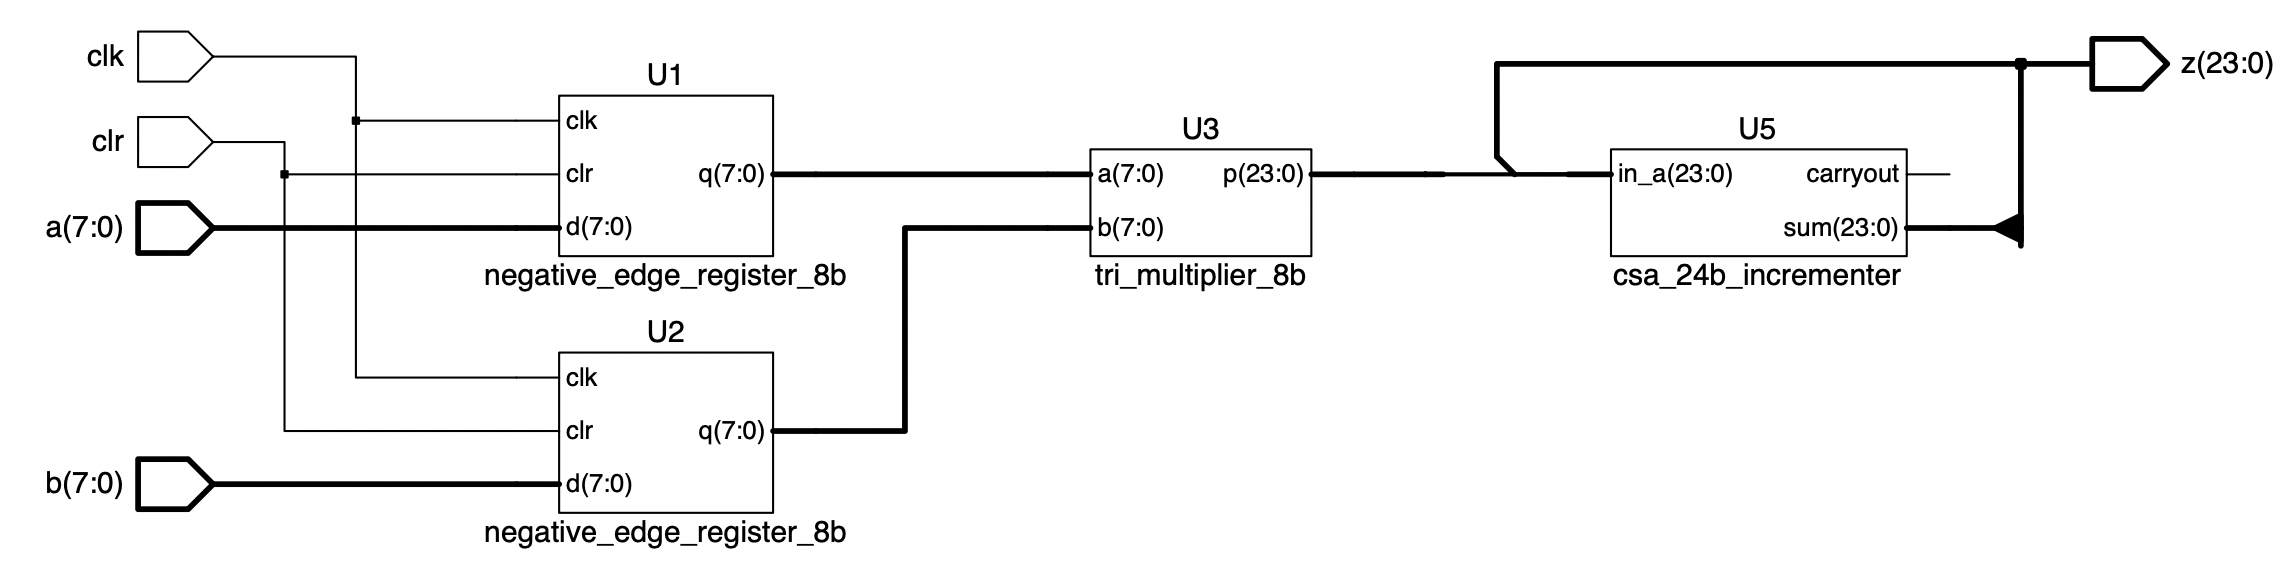
\includegraphics[width=\textwidth]{../img/non_p_op_rtl.png}
	\label{fig:non_p_op_rtl}
\end{figure}

The test simulation results for the non-pipelined operating circuit are shown in \figref{fig:non_p_op_sim}.

\begin{figure}[!htp]
	\centering
	\caption{Simulation Wave Diagram of Non-pipelined Operating Circuit}
	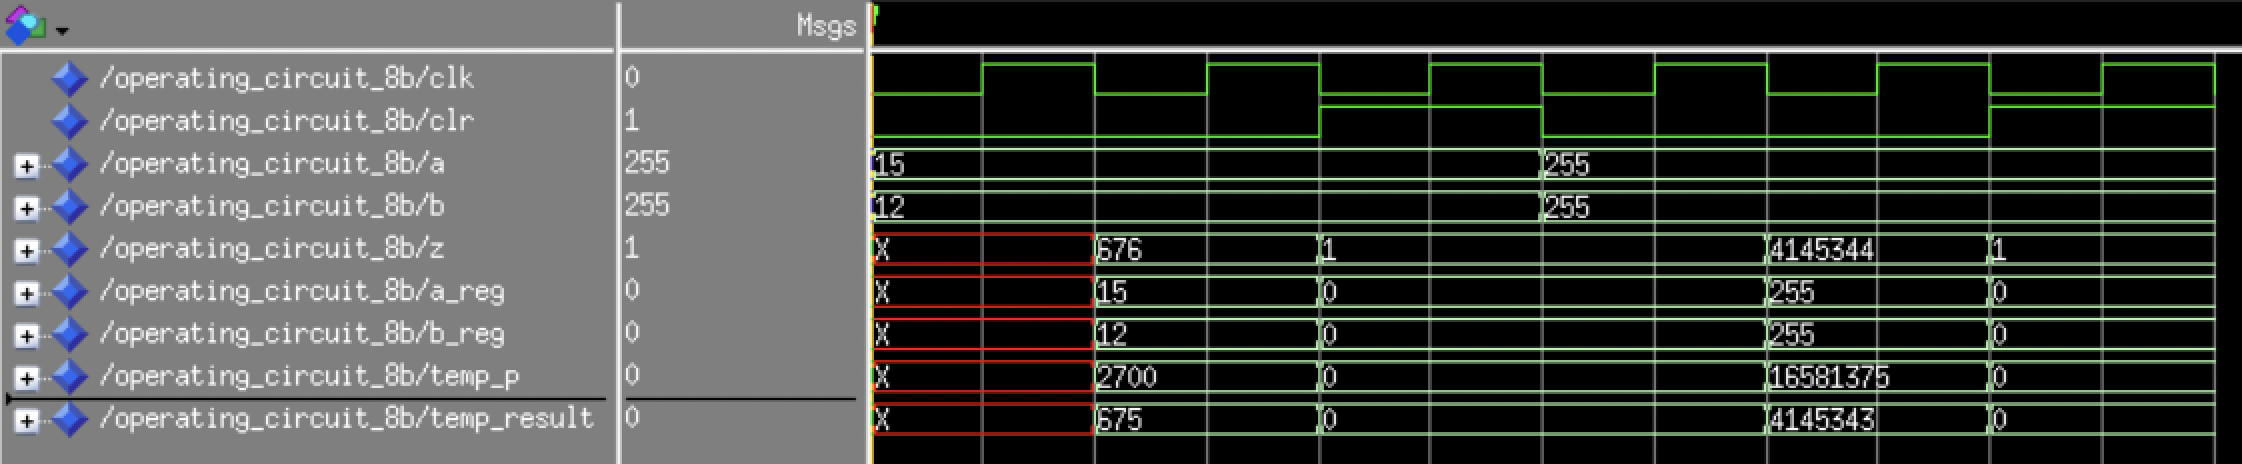
\includegraphics[width=0.9\textwidth]{../img/non_p_op_sim.png}
	\label{fig:non_p_op_sim}
\end{figure}

\subsection{Output Process}

In the non-pipelined implementation, negation output is used to meet the project requirements of 16-bit Z-port outputs,
which just represent the result as overflow.
The implementation of the whole circuit is shown in \figref{fig:non_p_rtl}.
The test simulation results for the negation output are shown in \figref{fig:non_p_sim}

\begin{figure}[!htp]
	\centering
	\caption{Synthesized RTL Diagram of Non-pipelined Circuit}
	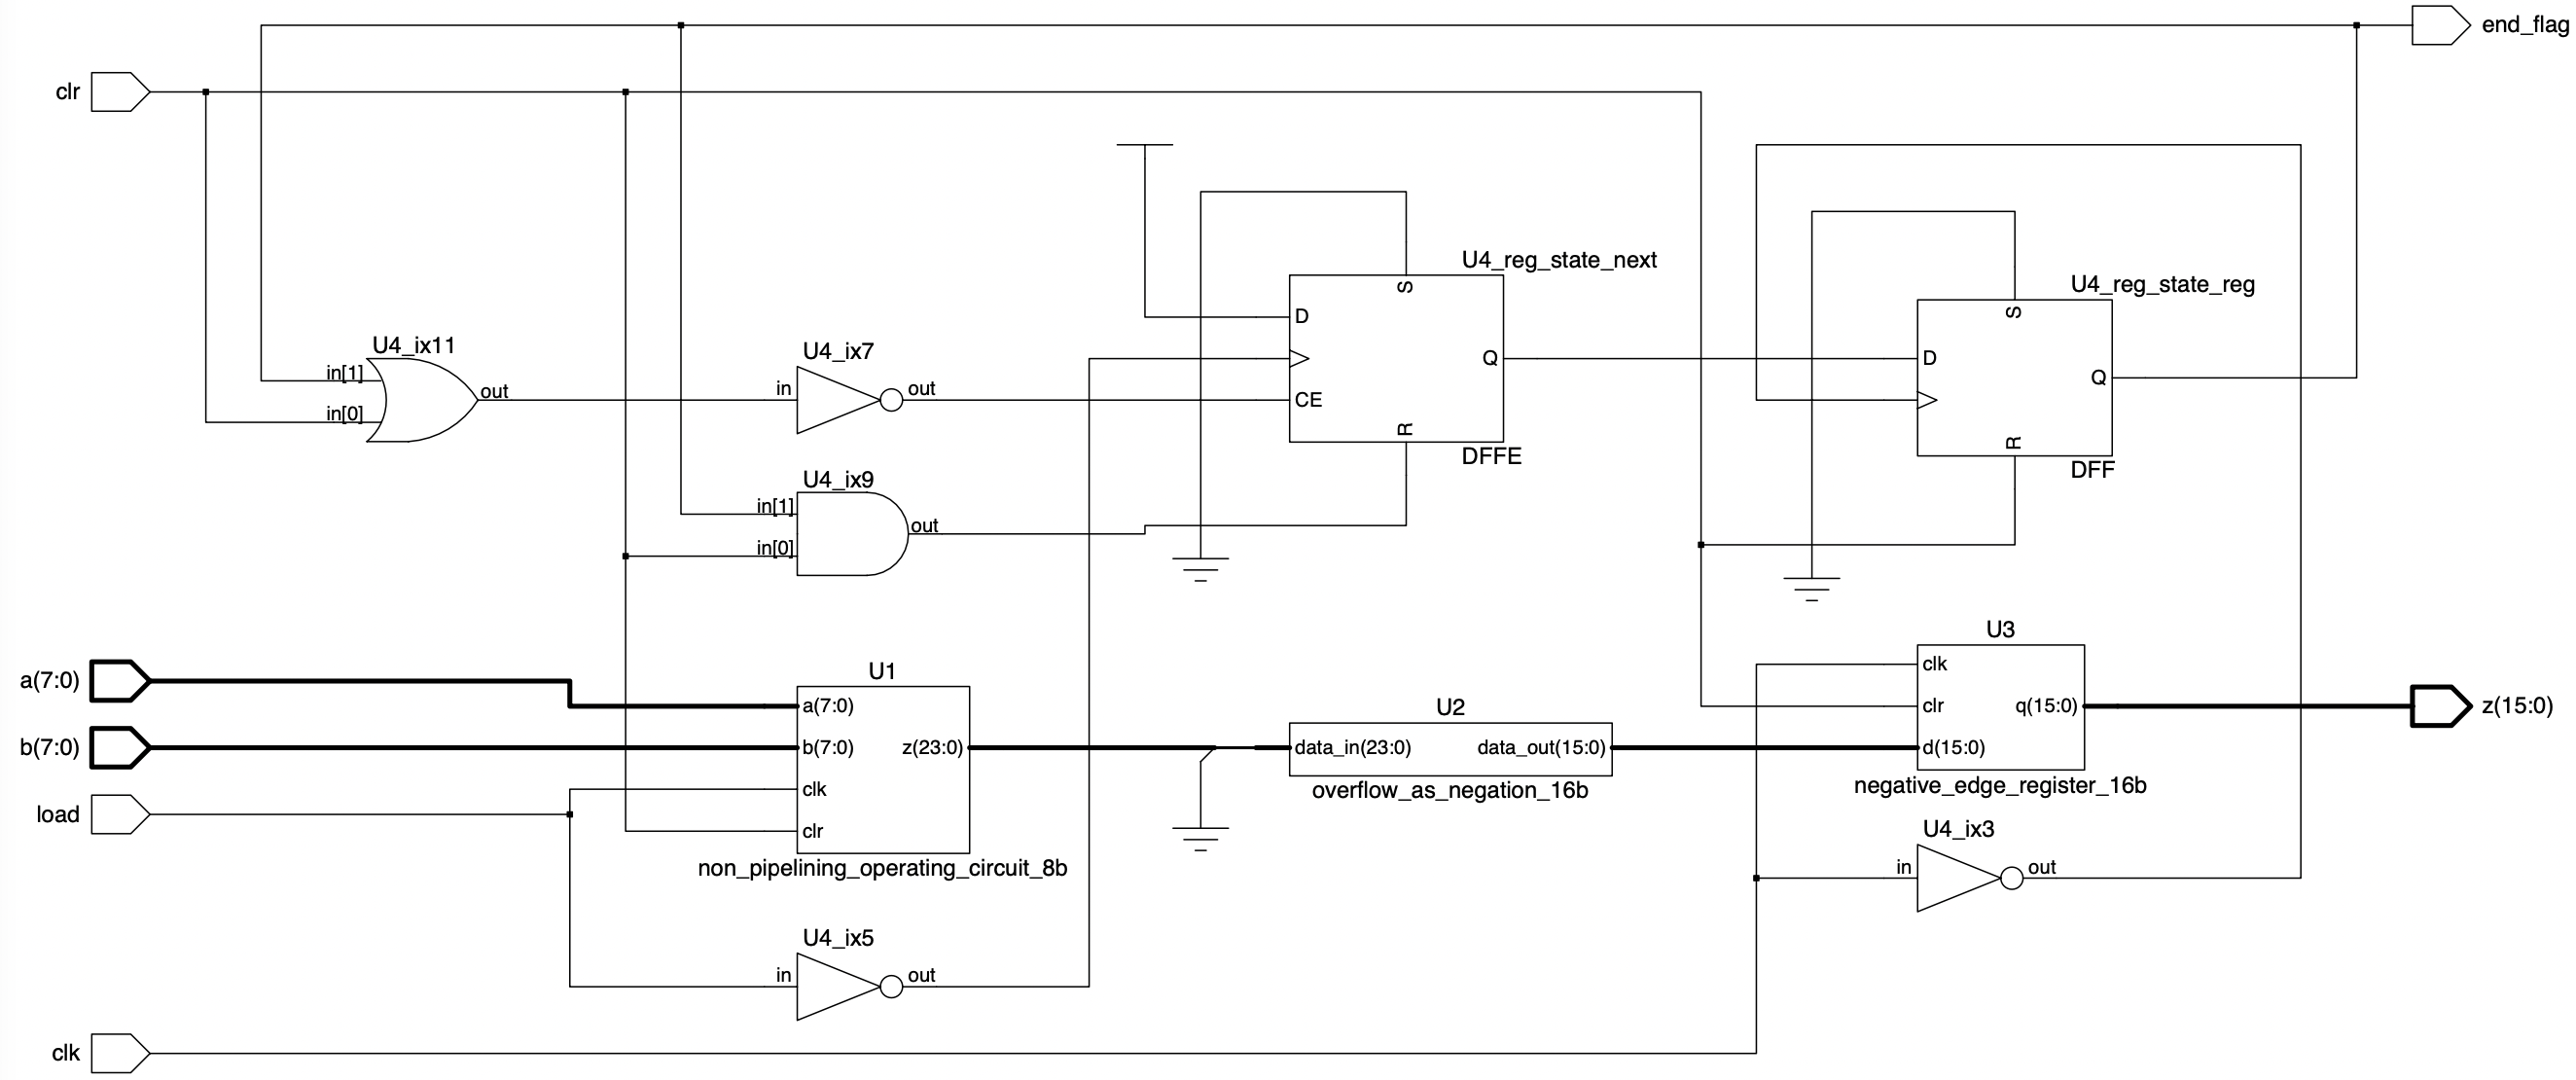
\includegraphics[width=\textwidth]{../img/non_p_rtl.png}
	\label{fig:non_p_rtl}
\end{figure}

\begin{figure}[!htp]
	\centering
	\caption{Simulation Wave Diagram of Non-pipelined Circuit}
	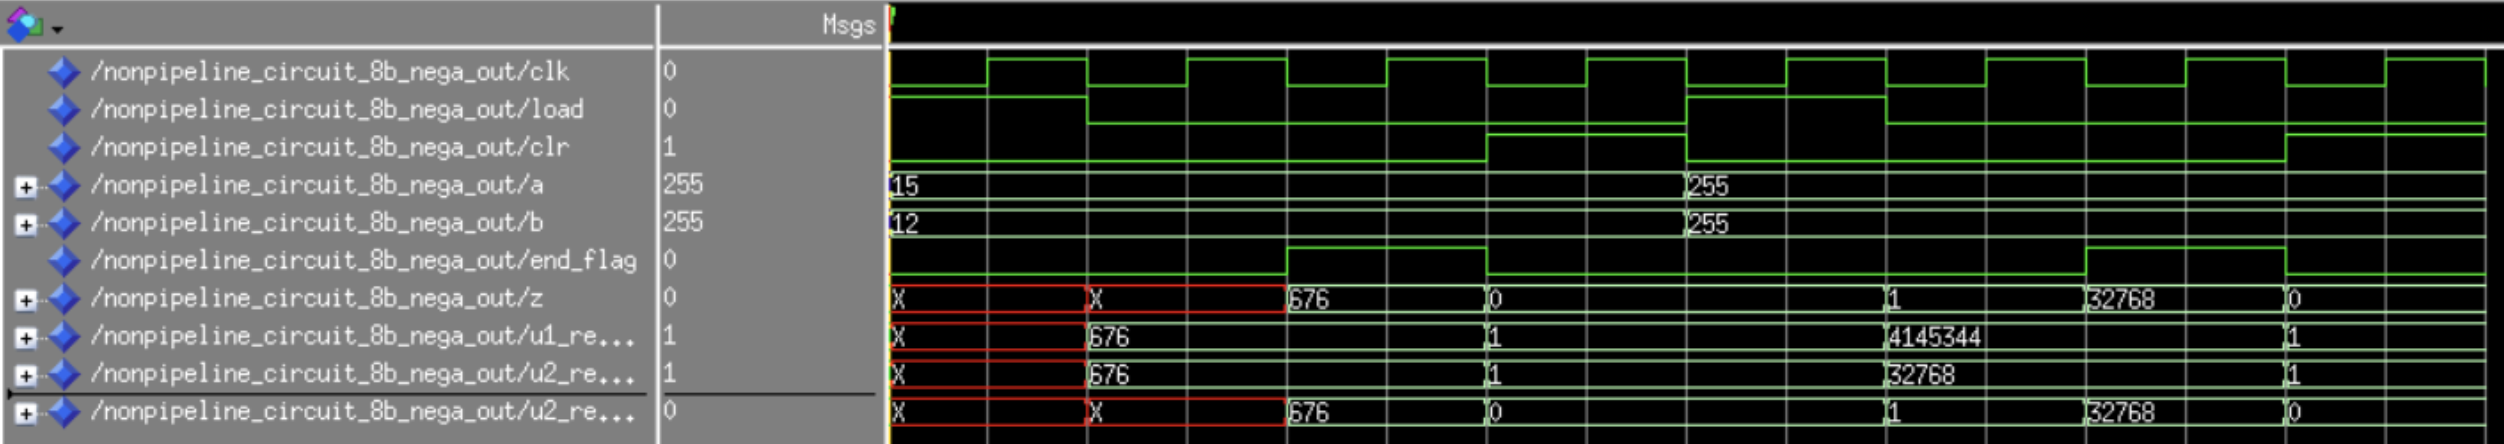
\includegraphics[width=0.9\textwidth]{../img/non_p_sim.png}
	\label{fig:non_p_sim}
\end{figure}
